% ---------------------------------------------------------------------------
% Response to R2 Major 1 / R1 Major 2 -- JEDC revision
%
% Upload this file together with FIGURE_decomposition.jpg to Overleaf and
% compile with pdfLaTeX. Only standard packages are used.
%
% To paste into an existing response document instead, take everything
% between the "BODY BEGINS" and "BODY ENDS" markers below.
% ---------------------------------------------------------------------------
\documentclass[11pt]{article}

\usepackage[utf8]{inputenc}
\usepackage[T1]{fontenc}
\usepackage{lmodern}
\usepackage[margin=1in]{geometry}
\usepackage{graphicx}
\usepackage{booktabs}
\usepackage{amsmath}
\usepackage{csquotes}
\usepackage{microtype}
\usepackage[hidelinks]{hyperref}

\setlength{\parskip}{0.6em}
\setlength{\parindent}{0pt}

% quotation block for the suggested manuscript wording
\usepackage{framed}
\usepackage{xcolor}
\colorlet{shadecolor}{gray!12}

\title{\textbf{R2, Major 1 \quad and \quad R1, Major 2}\\[0.3em]
       \large\normalfont\itshape Is it uncertainty, or just dearer oil?}
\author{}
\date{}

\begin{document}
\maketitle
\vspace{-3em}

% =========================== BODY BEGINS ===================================

Both referees raise the same point, and they are right. In our model, when oil
prices become more volatile, two things happen at the same time. The range of
prices the country might face next quarter gets wider --- that is the
uncertainty we set out to study. But the price it expects to pay also goes up.
We had been calling both of these ``uncertainty,'' which runs two separate things
together.

So we built the economy the referees asked for: one where the expected oil price
does not change as volatility rises, while the range of possible prices around
it still widens.
Everything else is held fixed --- same grid, same parameters, same shocks.

Writing $z$ for the log oil price and $v$ for the variance of next quarter's
price innovation, which is what rises with volatility, the corrected economy
draws
\[
  z' = (1-\rho)\bar{z} + \rho z - \tfrac{1}{2}\left(v - \bar{v}\right)
       + \sqrt{v}\, u',
  \qquad \bar{v} = \mathrm{E}[v].
\]
The original model is the same line without the $-\tfrac{1}{2}(v-\bar{v})$
term. That term is exactly the lift that pushes up the expected \emph{level} of
the price when the mean of its logarithm is unchanged, so subtracting it holds
the expected price fixed while leaving the spread of possible prices free to
widen. We centre the correction on the average variance rather than on zero so
that the corrected economy lines up with the constant-volatility economy we
compare it against.

It behaves as it should: in the original model the expected price climbs about
1.8\% as we move from the calmest conditions to the most turbulent, while in the
new one it does not move at all (Figure~\ref{fig:decomp}a).

\section*{Uncertainty does matter on its own}

The clearest way to see this is to stay inside that new economy and compare its
calm periods with its turbulent ones. The expected oil price is the same in
both, so anything that changes across them must be caused by uncertainty.

\begin{table}[h]
\centering
\small
\begin{tabular}{lcccc}
\toprule
when oil prices are\ldots & how volatile & spread & chance of default each year & average oil price \\
\midrule
calmest          & 0.09 & 330 bp         & 2.2\%            & 1.247 \\
                 & 0.11 & 337            & 2.7              & 1.248 \\
                 & 0.13 & 350            & 3.1              & 1.241 \\
                 & 0.17 & 363            & 3.9              & 1.239 \\
most turbulent   & 0.21 & \textbf{377}   & \textbf{5.1}     & 1.228 \\
\bottomrule
\end{tabular}
\end{table}

Both measures climb steadily. Spreads rise by 47 basis points, and the chance of
default each year more than doubles, from about 2\% to 5\%. The important column is
the last one: the average oil price is \emph{lower} in the turbulent
periods, not higher. The country is paying less for its oil and defaulting more
often anyway. There is no way to tell that story as an expected-price effect.

To be sure this is not simulation noise, we ran the same comparison in the
constant-volatility economy, where volatility never changes, so its five
``states'' are the same thing five times over and nothing should move across
them. Across those, spreads move by less than one basis point and default rates
by about a tenth of a percentage point --- a small fraction of the swings above.
So uncertainty on its own raises both what the country pays to borrow and how
often it defaults, and this is what we now lead with in Section 6.3.

\section*{What the averages say}

Averaged over the whole simulation, the referees' point applies in full, and we
would rather state that plainly than soften it. Oil price risk in total matters a
great deal to these countries: it accounts for 200.7 basis points of the average
spread, roughly half of it. But the part that comes from volatility
\emph{changing over time} is small, about 13 basis points --- and when we split
that in two, most of it, 12 of the 13, is the expected-price effect rather than
uncertainty. That is exactly what R2 suspected.

We report this but do not build the section on it, for a reason we should state
openly. Our correction is exact one quarter ahead, but these are long
bonds, priced over something closer to six years, and over that longer horizon it
drifts and overcorrects --- which makes the expected-price share look
too large and the uncertainty share too small. So we read the 12 as a ceiling
and the 1.3 as a floor rather than as a measurement. The comparison in the
previous section is free of this, because it never sets one economy against
another. We have also cut a line from our first draft calling the price effect
``thirty times'' the volatility effect; it invited a comparison the numbers
cannot carry.

\section*{Borrowing}

R1 asks the natural follow-up: with the expected-price effect taken out, does
the country still borrow less when things get risky? We looked at the borrowing
decisions directly, holding income and existing debt fixed so that volatility is
the only thing changing. In the original model, higher volatility leads the
country to pay down debt in nine of the sixty-nine situations we can resolve;
with the correction, that falls to three (Figure~\ref{fig:decomp}c). So most of
the reduction in borrowing was a response to expecting dearer oil, but not all
of it. An
earlier draft of this response claimed those cases vanished entirely --- they do
not, and we were wrong about that. What is left is too thin for us to claim a
general precautionary motive either way.

\begin{figure}[htbp]
\centering
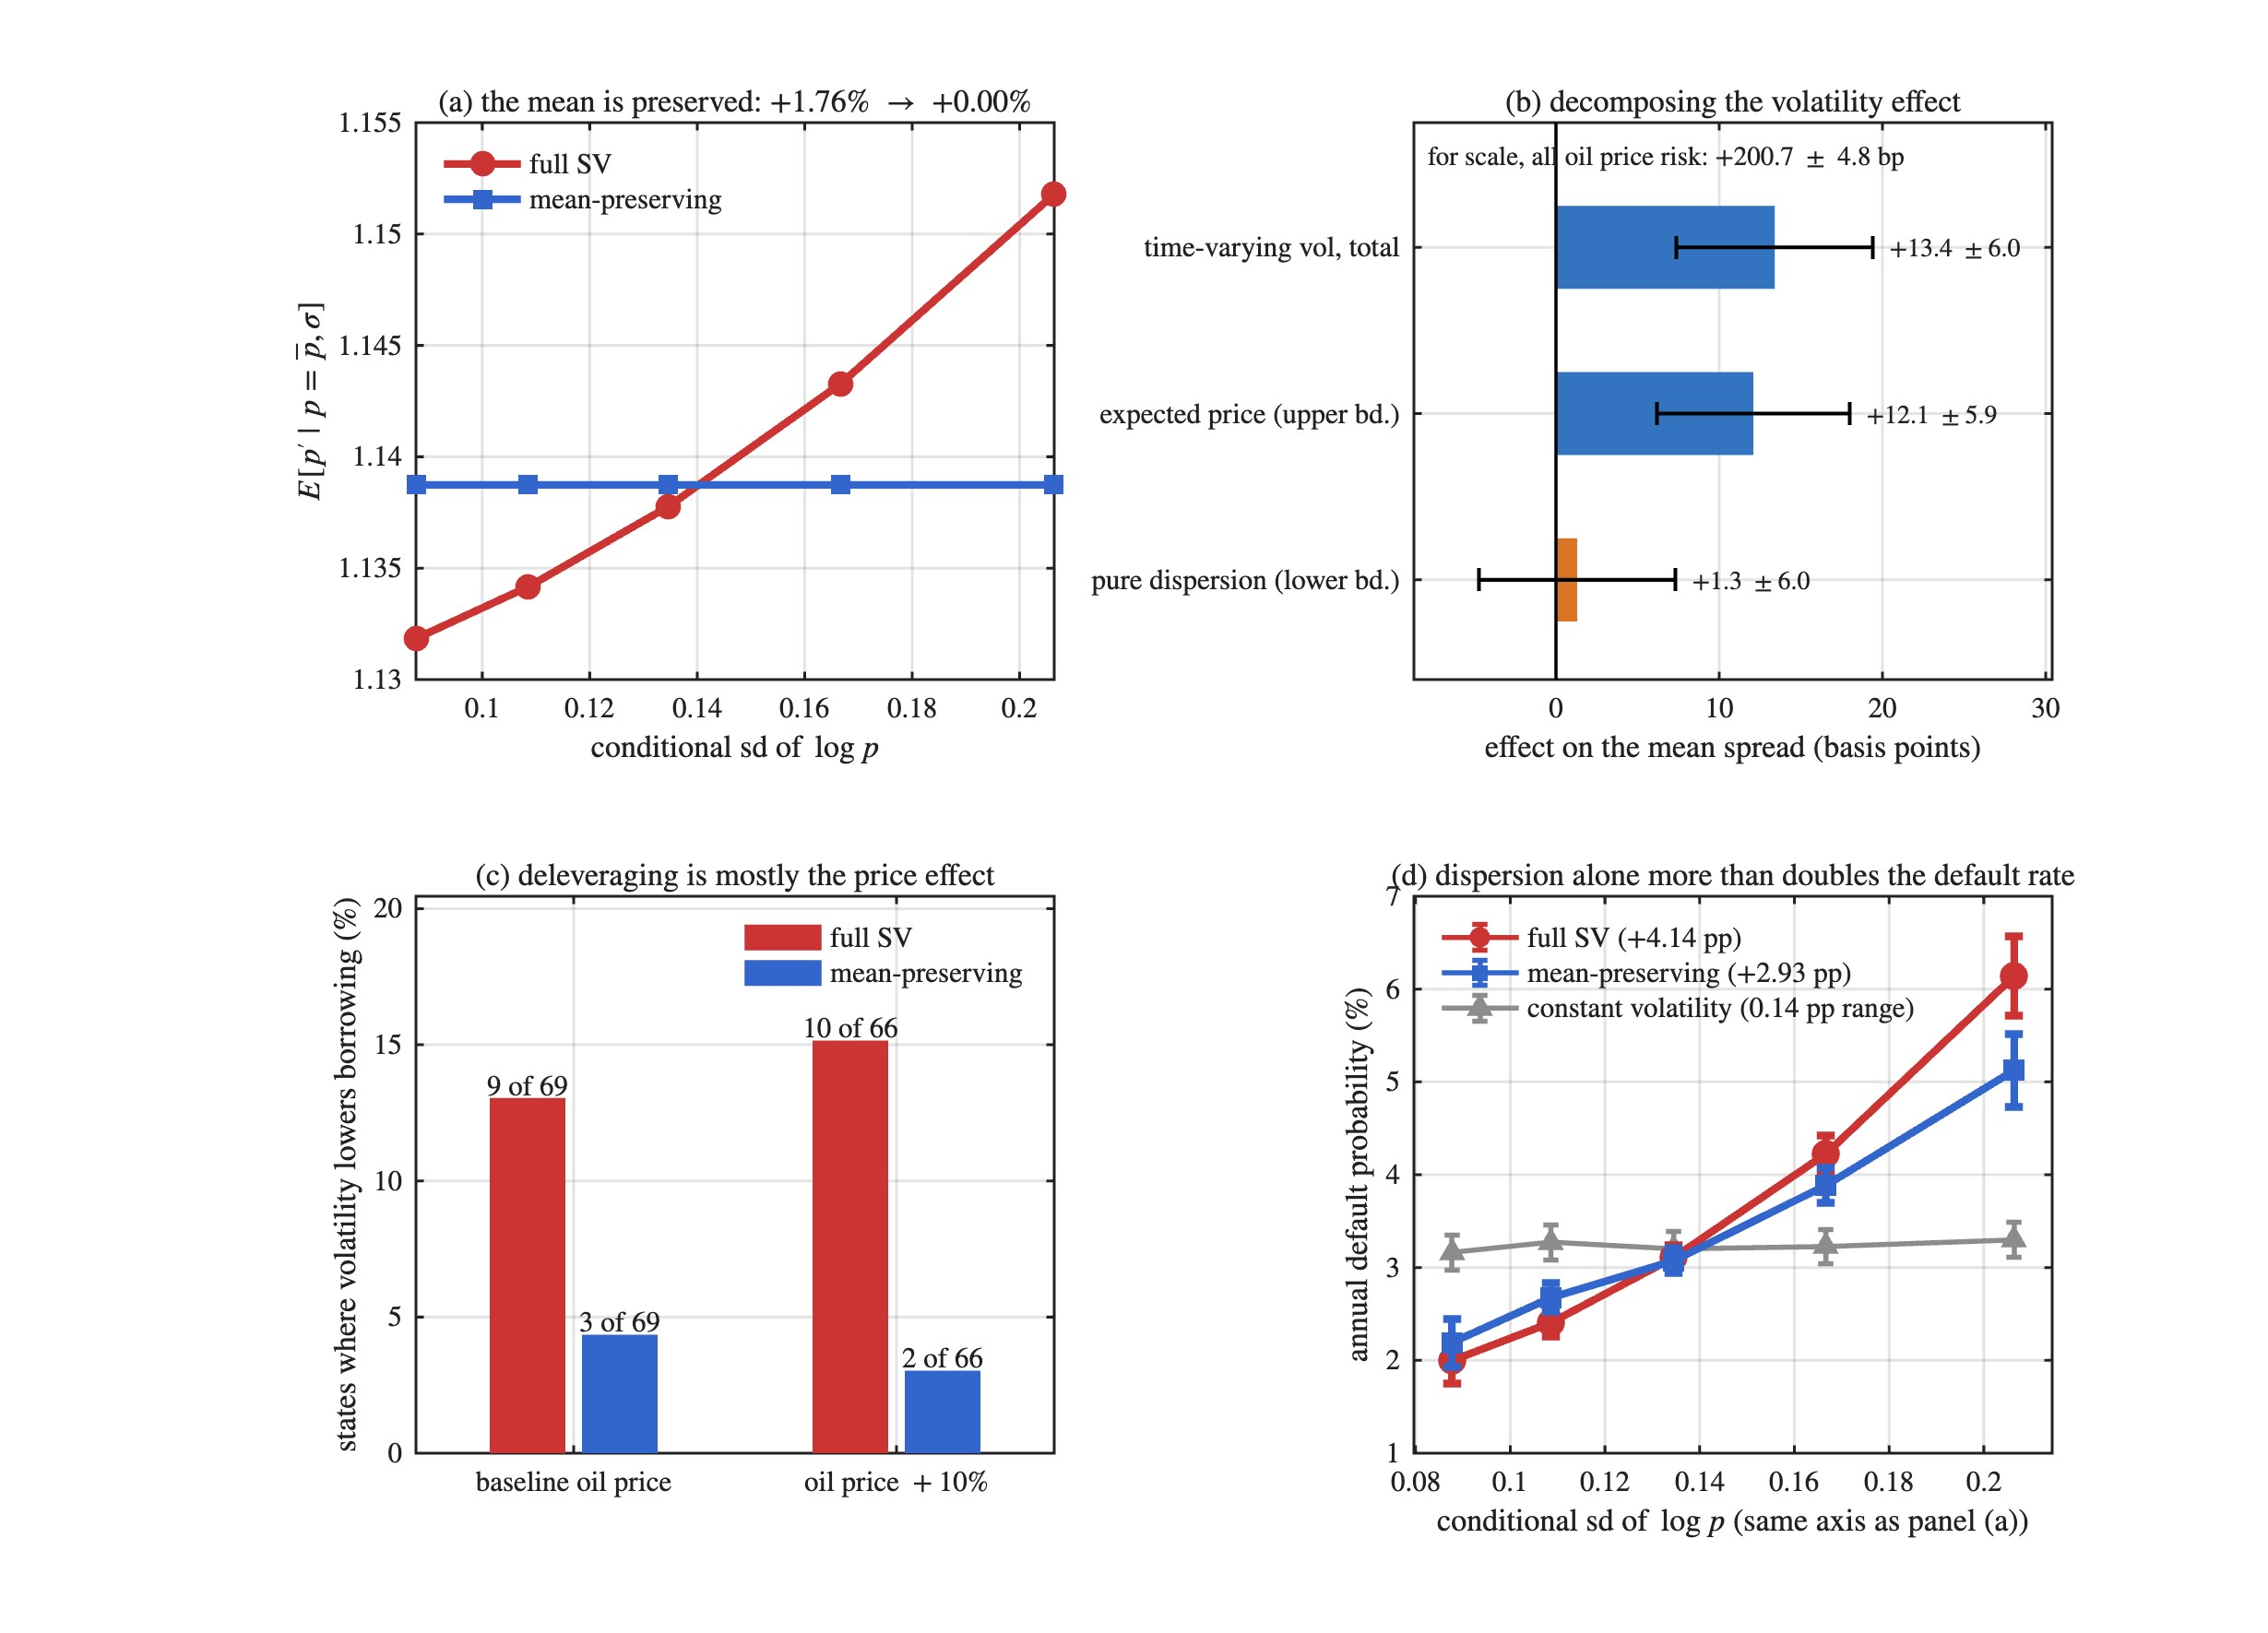
\includegraphics[width=\textwidth]{FIGURE_decomposition.jpg}
\caption{\textbf{(a)} The expected oil price next quarter, by how volatile
prices currently are, in the original model and in the corrected one.
\textbf{(b)} What time-varying volatility does to the average spread, and how
that divides between expected prices and dispersion. The bars carry 95\%
simulation intervals; a bar whose interval crosses the zero line cannot be told
apart from zero. The effect of oil price risk as a whole is far larger, at
$+200.7$ basis points, so it is written in rather than drawn, to keep the three
smaller bars readable. \textbf{(c)} How often higher volatility leads the
country to borrow less, at the baseline oil price and after a 10\% rise.
\textbf{(d)} The annual chance of default by volatility, on the same scale as
panel (a). Panels (a) and (d) are the whole exercise in one picture: the
expected price is flat across the corrected economy's volatility states, its
default rate still more than doubles, and the constant-volatility economy
stays flat throughout.}
\label{fig:decomp}
\end{figure}

We have rewritten Section 6.3 along these lines. R2 writes that a small
pure-uncertainty effect would be a perfectly good answer, so long as the reader
comes away understanding why volatility matters. We think that is where we have
ended up. The comment cost us a headline claim, and the paper is better for it. We thank
the referees for raising it.

\bigskip
\hrule
\bigskip

\subsection*{Suggested manuscript wording}

\begin{shaded}
\noindent
We separate the two effects of oil price volatility by solving an economy in
which the expected price is held fixed while its dispersion still varies. Within
that economy, spreads rise steadily by 47 basis points and the annual default
probability from 2.2\% to 5.1\% between the calmest and most turbulent
conditions, while the average oil price falls; the constant-volatility economy
moves by less than a basis point and a tenth of a percentage point across the
same states. Uncertainty therefore raises both the cost of borrowing and the
incidence of default. Averaged over the simulation, oil price risk as a whole
accounts for 200.7 basis points of the spread and time variation in volatility
for a further 13, of which roughly 12 is attributable to expected prices and 1
to dispersion; because the adjustment is exact only one quarter ahead and
overstates itself at the horizons relevant for long-term debt, we read these as
a ceiling and a floor rather than a measured split. Reductions in borrowing
become three to five times less common once the expected-price effect is
removed, but do not disappear.
\end{shaded}

\subsection*{Note}

The derivations, the quarter-by-quarter behaviour of the correction, the full
tables and the sensitivity to the substitution elasticity are all in
\texttt{results/response\_R2M1\_R1M2\_FULL\_DETAIL.md}, which we are happy to
provide. Every number here comes from
\texttt{model/economies\_common\_check/}, four separate Fortran programs solved
on a common price grid; the tables and the figure are produced by a single
MATLAB file, \texttt{model/analysis/JEDC\_decomposition.m}, and written to
\texttt{model/economies\_common\_check/decomposition/}.

% ============================ BODY ENDS ====================================

\end{document}
